% IEEE Conference Format — IEEEtran
\documentclass[conference]{IEEEtran}
\IEEEoverridecommandlockouts

\usepackage[utf8]{inputenc}
\usepackage[T1]{fontenc}
\usepackage{amsmath}
\usepackage{amssymb}
\usepackage{graphicx}
\usepackage{booktabs}
\usepackage{array}
\usepackage{multirow}
\usepackage[hyphens]{url}
\usepackage{cite}
\usepackage{tabularx}
\usepackage{microtype}
\usepackage{float}
\usepackage[hidelinks, breaklinks=true]{hyperref}

% Relax justification to reduce underfull/overfull hbox warnings
\tolerance=3000
\emergencystretch=20pt
\hbadness=10000

\graphicspath{{figures/}{latex/figures/}}

% -------------------------------------------------------
\begin{document}

\title{Privacy-Preserving NZSL/BSL Fingerspelling Recognition Using Skeleton Keypoints}

\author{%
  \IEEEauthorblockN{19069041 PAL, Harmandeep \quad 25319733 WEN, Man \quad 25293800 DHILLON, Darashveer Singh}
  \IEEEauthorblockA{\{zdh3114, xzw4582, mtz4764\}@autuni.ac.nz\\
    COMP820 -- Video and Image Processing\\
    Auckland University of Technology}
}

\maketitle

% -------------------------------------------------------
\begin{abstract}
This study presents a privacy-preserving fingerspelling recognition system for the New Zealand Sign Language (NZSL) and British Sign Language (BSL) alphabet and numbers. Rather than processing raw images, the system uses MediaPipe to extract hand skeleton keypoints, which are immediately discarded after extraction so that no personal visual information is retained at inference time. Each image is converted into a 508-dimensional geometric feature vector encoding wrist-relative coordinates, pairwise landmark distances, and hand orientation. To handle the structural difference between one-handed and two-handed signs, the system trains separate models for each group and automatically routes predictions at inference based on the number of hands detected. Five classifiers were evaluated: SVM, Random Forest, k-NN, Scikit-learn MLP, and Keras MLP, all achieving above 99\% accuracy on a 34-class test set. The keypoint-based SVM outperformed a raw-pixel baseline by approximately 3.5 percentage points (99.87\% vs 96.33\%), demonstrating that removing personal visual information does not reduce accuracy but improves it. A hard-pair analysis was also conducted on real-world problematic sign pairs such as L/A, T/A, U/S, and U/E to evaluate the system's ability to distinguish these signs. The system is deployed as a live web demo, confirming its suitability for real-time use.
\end{abstract}

\begin{IEEEkeywords}
sign language recognition, fingerspelling, skeleton keypoints, privacy-preserving, MediaPipe, NZSL, BSL, SVM, machine learning
\end{IEEEkeywords}

% -------------------------------------------------------
\section{Introduction}

In recent years, the rapid development of digital technologies has made data collection common in many fields. As a result, privacy protection has become an increasingly important issue, especially for image data that contains human-related information. Sign language and gesture images are particularly sensitive because they may include not only hand gestures, but also faces, body posture, clothing, and background details. These visual features can reveal a person's identity and may also expose personal habits or behavioural information.

For example, sign language is an important communication method for Deaf and hard-of-hearing communities. Sign language videos often contain facial expressions and hand movements, which are useful for linguistic analysis. However, if these videos are used directly without preprocessing, they may create a risk of identity leakage. Moreover, the widespread use of databases and online platforms has increased the possibility of video data being shared, stored, or reused in different contexts. Therefore, when studying sign language linguistics, it is important to protect privacy while keeping useful gesture information~\cite{rathmann2025}.
HMM
Figure~\ref{fig:bsl} illustrates static fingerspelling gestures from the British Sign Language (BSL) alphabet, which belongs to the BANZSL (British-Australian-New Zealand Sign Language) language family. This type of visual data is relevant to this project because BSL and New Zealand Sign Language (NZSL) share historical connections within the BANZSL family, and both involve hand-based alphabet signs that may require privacy-preserving preprocessing..

\begin{figure}[ht]
  \centering
  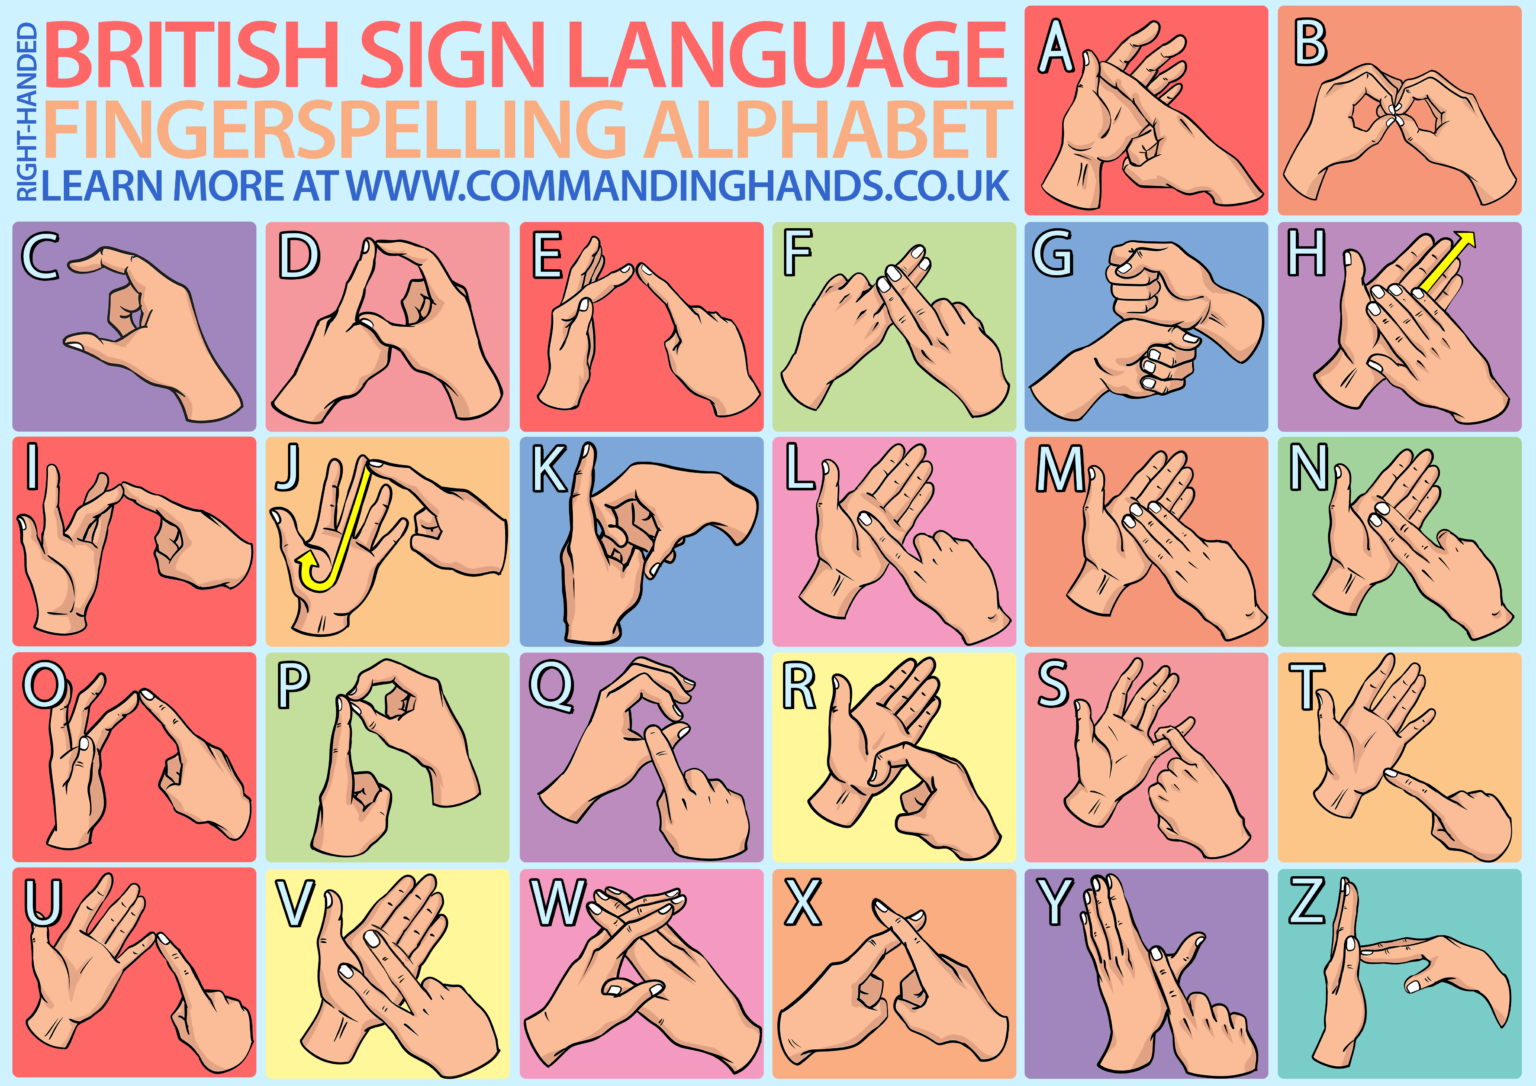
\includegraphics[width=\columnwidth]{image3.png}
  \caption{BSL alphabet chart. Source: commandinghands.co.uk}
  \label{fig:bsl}
\end{figure}

This study aims to develop a preprocessing tool for static sign language images and image datasets. The main purpose of the tool is to reduce privacy risks while preserving useful gesture-related information for later recognition and analysis. Instead of using raw images directly, this study explores a safer way to prepare data before it is used for training, testing, or demonstration. This process can help protect personal privacy and provide cleaner and more reliable data for future sign language recognition tasks. This leads to the following research question.

\textbf{RQ:} How can a privacy-preserving, real-time fingerspelling recognition system be designed to accurately classify both one-handed and two-handed signs across the full NZSL/BSL alphabet and numbers?

% -------------------------------------------------------
\section{Literature Review}

\subsection{Sign Language and Gesture Recognition}

Sign language recognition has become an important research direction in computer vision and pattern recognition. It supports communication accessibility for Deaf and hard-of-hearing people and also contributes to human-computer interaction. Existing studies have explored different methods, including handcrafted feature extraction, Convolutional Neural Network (CNN)-based image classification, CNN-LSTM or CNN-BiLSTM models, attention-based networks, MediaPipe landmark extraction, and YOLO-based real-time detection.

Early recognition methods often relied on sensor-based devices or handcrafted image features such as SIFT and HOG. However, these methods can be affected by hardware dependency, lighting changes, background noise, and occlusion~\cite{ghous2025}. With the development of deep learning, CNN-based models have been widely used to extract spatial features from hand images, while Long Short-Term Memory (LSTM) or BiLSTM models are often used to capture temporal information in dynamic gestures. For example, Min et al.~\cite{min2025asl} proposed a multi-scale CNN and BiLSTM-based ASL recognition system using MediaPipe preprocessing and attention-based feature learning. YOLO-based methods have also been applied to real-time hand detection and gesture localisation. Fu et al.~\cite{fu2025} used an improved YOLOv8 model for Tibetan sign language recognition, while Ghous et al.~\cite{ghous2025} combined YOLO-based hand keypoint detection with feature fusion and Hidden Markov Model (HMM) based temporal classification. However, these studies mainly focus on recognition accuracy and real-time performance, while the privacy risks in raw image data are often not fully addressed.

\subsection{Privacy Protection in Image Data}

Privacy protection is an important issue in image and video data because this type of data may contain identifiable information, such as faces, body movements, clothing, background environments, and voices. Golann et al.~\cite{golann2026} explain that large video datasets can create ethical, methodological, and technical challenges, especially when data are stored, shared, or reused by different researchers. They also note that even publicly available video data can still raise ethical concerns if the people in the videos did not expect their images to be used for research.

This issue is more specific in sign language research. Rathmann et al.~\cite{rathmann2025} state that sign language data are collected through a visual-gestural form, which makes participant visibility and anonymity difficult to manage. Sign language videos often include the signer's face, hands, body posture, and movements. These features are useful for analysis, but they may also expose the signer's identity. Some implemented privacy protection methods include face blurring and using pseudonyms, though these often prove challenging. If too much visual information is removed, useful gesture information may also be lost. Therefore, privacy protection should reduce identifiable information while preserving useful hand and gesture features.

\subsection{Skeleton-based Hand Features and Research Gap}

Skeleton-based hand features provide a useful way to balance privacy protection and gesture information preservation. Instead of using the full raw image, skeleton-based methods use key points to describe the structure and movement of the hands or body. For sign language images, hand landmarks are important because they can show finger positions, hand shapes, and spatial relationships between joints. This representation can keep useful gesture information while reducing the need to use original images directly.

Min et al.~\cite{min2025skeleton} explain that skeleton-based sign language recognition is a promising alternative to video-based methods because skeleton data can reduce visual noise, lower computational cost, and improve privacy protection. MediaPipe provides a practical way to generate this type of hand feature. Singh \& Gupta~\cite{singh2026} used MediaPipe to detect 21 landmarks per hand and saved the normalised landmark coordinates as training data. They also reported that no raw images or videos were stored, and only anonymised landmark vectors were saved locally.

Although previous studies have explored sign language recognition, image privacy protection, and skeleton-based features, these areas are often discussed separately. Many recognition systems focus on model performance without considering how image datasets should be safely prepared before training or deployment. This project addresses that gap by extracting keypoint hand data for model training, reducing privacy-sensitive visual information while preserving useful gesture features.

% -------------------------------------------------------
\section{Methodology}

\subsection{System Overview}

This study proposes a privacy-preserving fingerspelling recognition pipeline using static alphabet gestures from the BANZSL language family. NZSL, BSL, and Auslan share historical links within this language family, and their fingerspelling systems have similar visual structures. Due to the limited availability of suitable NZSL static image datasets, this project uses BSL-style alphabet data as a practical dataset for developing and testing the proposed preprocessing and recognition pipeline. Rather than operating on raw pixel data, the system extracts skeletal hand landmarks using MediaPipe Hands~\cite{lugaresi2019}, converting each image into a structured numerical feature vector. This design separates recognition accuracy from raw image storage, protecting personal identity while remaining suitable for embedded and real-time deployment. As illustrated in Figure~\ref{fig:pipeline}, the pipeline proceeds through four sequential stages: feature extraction, dataset partitioning, model training (one-hand and two-hand branches), and evaluation. The detailed SWOT analysis is provided in Appendix~\ref{app:swot}.

\begin{figure}[ht]
  \centering
  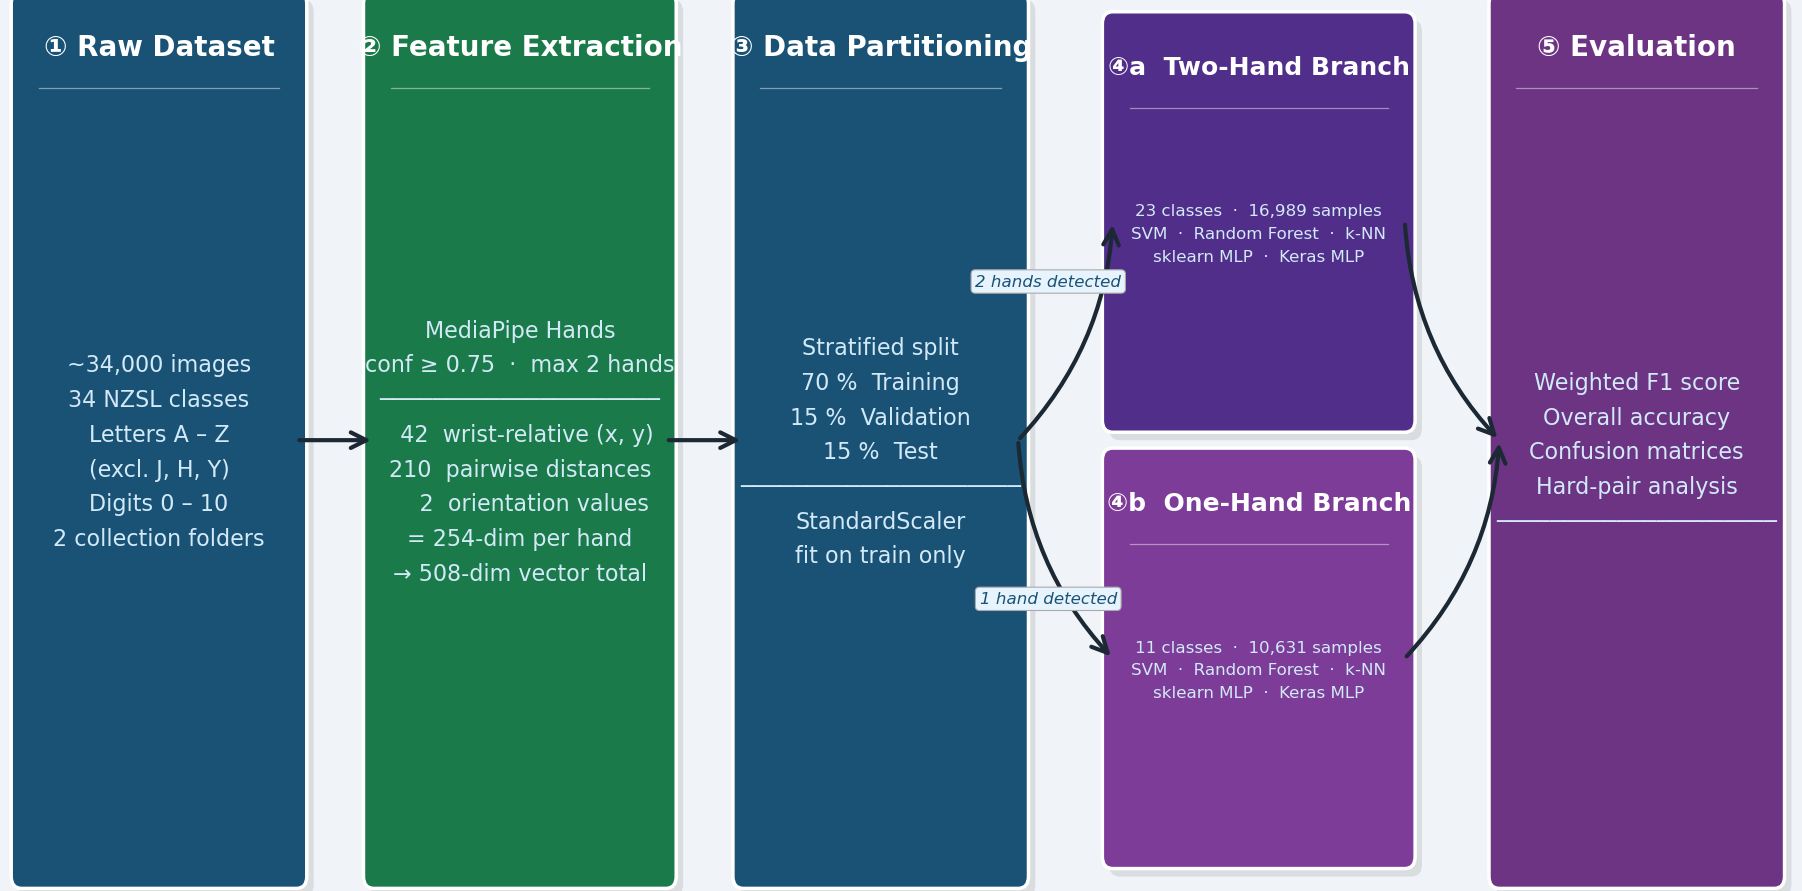
\includegraphics[width=\columnwidth]{image5.png}
  \caption{End-to-end pipeline for NZSL fingerspelling recognition.}
  \label{fig:pipeline}
\end{figure}

\subsection{Dataset and Class Definition}

The dataset comprised approximately 34,000 images spanning 34 BANZSL-related fingerspelling classes: the letters A--Z (excluding J, H, and Y) and the digits 0--10~\cite{tastepe2024}. Images were sourced from a collection representing different hand sign conditions to promote variance. The signs H, J were excluded as they require dynamic hand movement and cannot be represented by a single static keypoint snapshot, while Y was not available in the dataset (Table~\ref{tab:class_dist}).

\begin{table*}[t]
  \caption{Class Distribution by Hand Group}
  \label{tab:class_dist}
  \centering
  \begin{tabular}{p{1.8cm} p{10cm} c c}
    \toprule
    \textbf{Hand Group} & \textbf{Classes} & \textbf{Count} & \textbf{Extracted Samples} \\
    \midrule
    One-hand & C, 0--9 & 11 & 10,631 \\
    Two-hand & A, B, D, E, F, G, I, K, L, M, N, O, P, Q, R, S, T, U, V, W, X, Z, 10 & 23 & 16,989 \\
    Total & & 34 & 27,620 \\
    \bottomrule
  \end{tabular}
\end{table*}

\begin{figure}[ht]
  \centering
  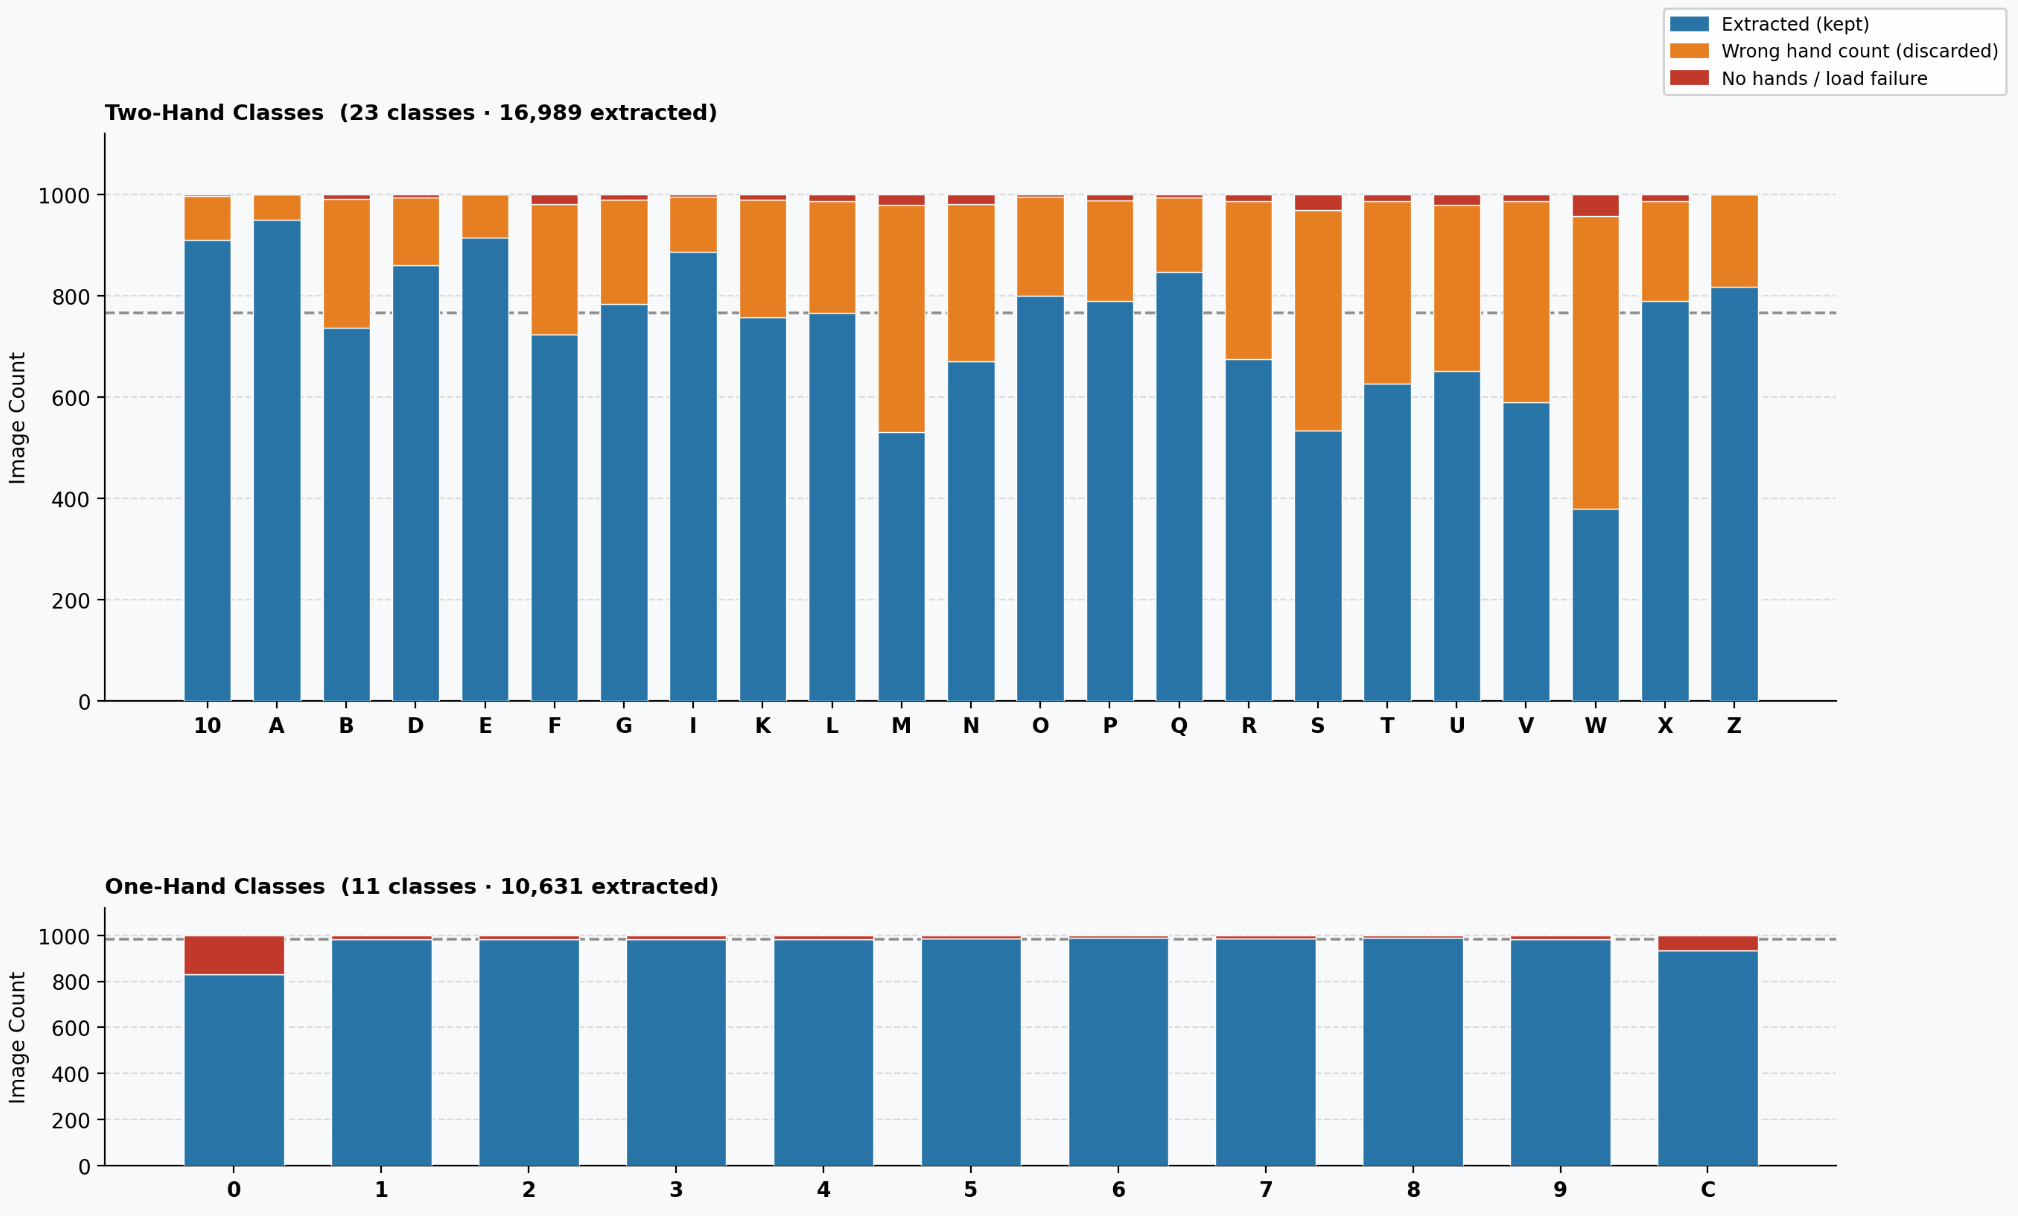
\includegraphics[width=\columnwidth]{image4.png}
  \caption{Per-class image yield after MediaPipe hand-landmark extraction.}
  \label{fig:yield}
\end{figure}

Although all classes initially contained 1,000 images, yield after landmark extraction varied considerably (Figure~\ref{fig:yield}). Class W, a two-handed sign requiring simultaneous detection of both hands yielded only 379 usable samples (379/1,000 = 62\% extraction failure rate), compared to $\geq$531 samples for all other classes. This shortfall is a consequence of MediaPipe's detection reliability rather than an intentional sampling decision.

\subsection{Feature Extraction}

Hand landmarks were detected using MediaPipe Hands with a minimum detection confidence of 0.75 and a maximum of two coexisting hands. For each detected hand, 21 landmarks were extracted and processed into a 254-dimensional feature vector comprising:
\begin{itemize}
  \item 42 wrist-relative coordinates: each landmark's (x, y) position translated to the wrist origin and normalised by palm scale (wrist-to-middle-finger-MCP distance);
  \item 210 pairwise Euclidean distances: all unique inter-landmark distances, providing scale-invariant shape descriptors;
  \item 2 orientation values: sine and cosine of the hand's principal axis angle, encoding rotational pose.
\end{itemize}

Both hands were always represented: if one hand was absent, its 254-dimensional slot was zero-padded. The final concatenated feature vector was always 508 dimensions, ensuring a consistent input shape regardless of sign type and enabling routing logic at inference time.

\begin{table*}[t]
  \caption{Model Configurations}
  \label{tab:models}
  \centering
  \begin{tabular}{>{\raggedright\arraybackslash}p{2.2cm} >{\raggedright\arraybackslash}p{7cm} >{\raggedright\arraybackslash}p{6cm}}
    \toprule
    \textbf{Model} & \textbf{Key Hyperparameters} & \textbf{Tuning} \\
    \midrule
    Support Vector Machine (SVM) (RBF kernel) &
      C = 100 (Regularization Parameter); $\gamma$ (gamma) = scale; &
      Grid search over $C \in \{0.1, 1, 10, 100\}$; best C = 100 for both groups \\
    \addlinespace
    Random Forest &
      seed = 42 &
      Default Configuration \\
    \addlinespace
    k-Nearest Neighbours &
      k = 3 (neighbors); metric = Euclidean; &
      Grid search over k (neighbors); best k = 3 for both groups \\
    \addlinespace
    Scikit-learn Multilayer Perceptron (MLP) &
      Layers: 256 $>$ 128 $>$ 64; ReLU (Activation function); Adam (Optimizer); lr (Learning Rate) = 0.001; max\_iter (Maximum Iterations) = 300 &
      Default configuration; no lr tuning; no early stopping \\
    \addlinespace
    Keras MLP &
      Layers: 256 $>$ 128 $>$ 64; Dropout (rate = 0.3) after each hidden layer; Adam (Optimizer); lr (Learning Rate) = 0.001; epochs $\leq$ 20 &
      Default configuration; no lr or Dropout tuning; early stopping (patience = 4) \\
    \bottomrule
  \end{tabular}
\end{table*}

\subsection{Data Partitioning}

Extracted feature vectors were partitioned using stratified splitting to preserve representative per-class proportions~: 70\% training, 15\% validation, 15\% test. Stratification was applied within each hand group independently. To strictly prevent preprocessing data leakage, feature standardisation (zero mean, unit variance) was fitted exclusively on the training partition and applied consistently to the validation and test sets~\cite{alhammad2026}.

\subsection{Model Architectures and Training}

Five classifier types were trained independently for each hand group, yielding ten model configurations in total. Table~\ref{tab:models} summarises the architecture and key hyperparameters selected following grid-search cross-validation.

The Keras MLP applied Dropout (rate = 0.3) after each hidden layer except the last, compiled with sparse categorical cross-entropy loss and class-balanced sample weighting. Early stopping monitored validation loss to prevent overfitting; training converged at epoch 3 (one-hand) and epoch 6 (two-hand), well within the 20-epoch ceiling. No image-level augmentation was applied; natural variance across signers and capture angles was considered sufficient for static skeletal features.

Two limitations are acknowledged: The SVM grid search upper bound (C=100) and sklearn MLP fixed training budget are acknowledged limitations of the tuning process

\subsubsection{Class Imbalance Mitigation}

Table~\ref{tab:imbalance} summarises the strategy applied for each classifier.

\begin{table}[H]
  \caption{Class Imbalance Handling per Model}
  \label{tab:imbalance}
  \centering
  \begin{tabular}{>{\raggedright\arraybackslash}p{1.8cm} >{\raggedright\arraybackslash}p{2.8cm} >{\raggedright\arraybackslash}p{2.6cm}}
    \toprule
    \textbf{Model} & \textbf{Strategy} & \textbf{Mechanism} \\
    \midrule
    SVM &
      class\_weight= balanced &
      Loss penalty inversely proportional to class frequency \\
    \addlinespace
    Random Forest &
      class\_weight= balanced\_subsample &
      Rebalances within each bootstrap sample \\
    \addlinespace
    k-NN &
      weights= distance &
      Closer neighbours weighted more heavily \\
    \addlinespace
    Keras MLP &
      Compute\_class\_weight= balanced &
      Scales loss contribution of minority classes during backpropagation \\
    \addlinespace
    sklearn MLP &
      None applied &
      No native class weight support; raw imbalanced data used \\
    \bottomrule
  \end{tabular}
\end{table}

\subsection{Architectural Decisions and Code Iterations}

Table~\ref{tab:adr} summarises the two key architectural decisions made during development. Each emerged in response to a concrete problem encountered while building the system.

\begin{table*}[t]
  \caption{Key Architectural Decisions and Iterations}
  \label{tab:adr}
  \centering
  \begin{tabular}{p{3cm} p{4.5cm} p{4.5cm} p{4cm}}
    \toprule
    \textbf{ADR} & \textbf{Problem} & \textbf{Solution} & \textbf{Outcome} \\
    \midrule
    Privacy-Preserving Keypoints &
      Raw images contain personal information such as skin tone, lighting, and background that is irrelevant to sign recognition &
      Images are used only to extract hand skeleton coordinates, then discarded immediately --- the model never sees or stores the original photo &
      Accuracy improved by $\approx$3.5\% over the raw-pixel approach while removing all personal visual information from the pipeline \\
    \addlinespace
    One-Hand / Two-Hand Routing &
      Training one model across all signs caused confusion because one-hand and two-hand signs have fundamentally different structures &
      The system was split into two separate models, one for each hand group, with automatic routing at inference based on how many hands are detected &
      Signs are classified by the correct specialist hand group model without any manual selection \\
    \bottomrule
  \end{tabular}
\end{table*}

\subsection{Evaluation}

Each model was evaluated on its held-out test partition using weighted F1 score as the primary metric to account for class imbalance, supplemented by overall accuracy. Confusion matrices and per-class classification reports were generated for both hand groups. The metrics are provided in the Results whereas the confusion matrices for SVM (RBF), the best model are provided in Appendix~\ref{app:cm}.

Hard-to-distinguish sign pairs (L/A, T/A, U/S, and U/E) were examined through pairwise analysis. A raw-pixel baseline, an SVM trained on 64$\times$64 grayscale images with Principal Component Analysis (PCA) dimensionality reduction, was included to show the benefit of the landmark-based representation (Figure~\ref{fig:baseline_compare}).

\begin{figure}[H]
  \centering
  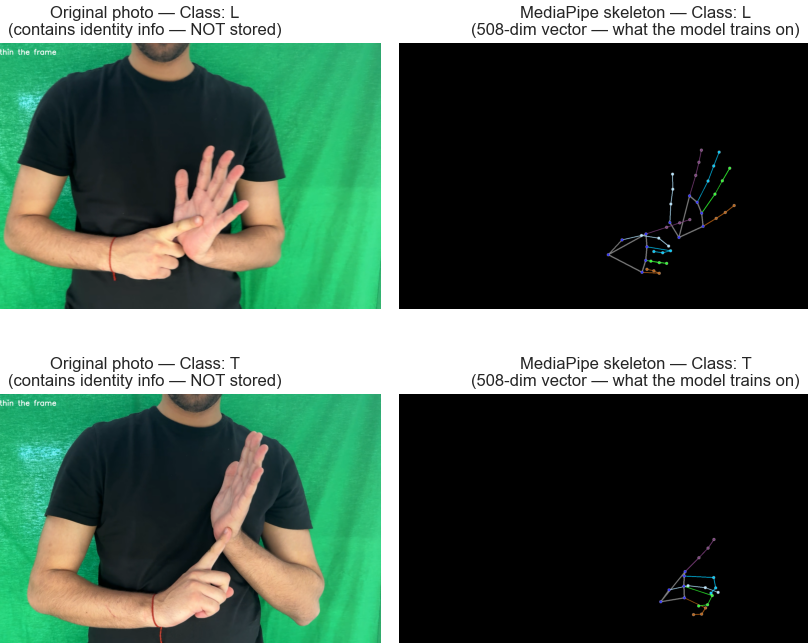
\includegraphics[width=\columnwidth]{image6.png}
  \caption{A raw-pixel baseline v/s Keypoints representation.}
  \label{fig:baseline_compare}
\end{figure}

% -------------------------------------------------------
\section{Results}

The initial results presented in this section evaluate the model on the primary dataset in a controlled environment. A subsequent analysis detailing its accuracy in a real-world environment is also provided.

\subsection{Privacy-Preserving Keypoint Approach vs Raw-Pixel Baseline}

To study the keypoint approach, a raw-pixel SVM baseline was trained on 64$\times$64 greyscale images with PCA dimensionality reduction across all 34 classes. Table~\ref{tab:baseline} compares the routed keypoint system against this baseline.

\begin{table}[ht]
  \caption{Keypoint System vs Raw-Pixel Baseline}
  \label{tab:baseline}
  \centering
  \begin{tabular}{p{2.5cm} c c p{1.5cm}}
    \toprule
    \textbf{Approach} & \textbf{Accuracy} & \textbf{Weighted F1} & \textbf{Raw Images at Inference} \\
    \midrule
    Keypoint SVM one-hand & 99.87\% & 99.87\% & No \\
    Keypoint SVM two-hand & 99.84\% & 99.84\% & No \\
    Raw-pixel SVM (baseline) & 96.33\% & 96.33\% & Yes \\
    \bottomrule
  \end{tabular}
\end{table}

The keypoint system outperforms the raw-pixel baseline by approximately 3.5 percentage points while requiring no raw image data at inference time. This confirms that landmark extraction not only preserves the privacy of the person but also improves classification accuracy, likely because the normalised geometric representation eliminates irrelevant variation in lighting, skin tone, and background. Figure~\ref{fig:keypoint_compare} extends this comparison across all models and shows that the 508-dimensional keypoint vector is substantially more compact than the PCA-reduced pixel representation, further reducing computational cost without sacrificing accuracy.

\begin{figure}[ht]
  \centering
  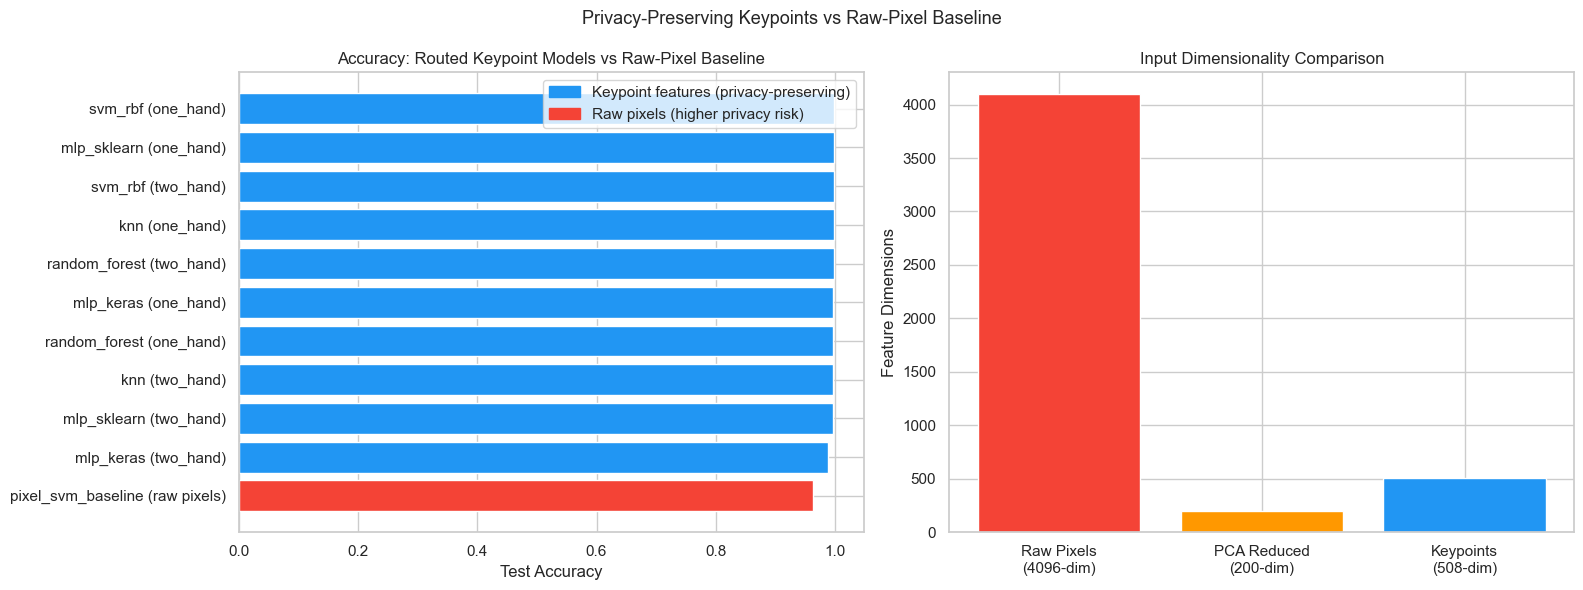
\includegraphics[width=\columnwidth]{image7.png}
  \caption{Privacy-Preserving Keypoints vs Raw-Pixel Baseline.}
  \label{fig:keypoint_compare}
\end{figure}

\subsection{Model Performance}

All five classifiers achieved high accuracy on both hand groups. Table~\ref{tab:performance} reports accuracy and weighted F1 score on the held-out test set (15\% stratified split) for each model and hand group, ranked by weighted F1 within each group.

\begin{table*}[t]
  \caption{Test Set Performance by Model and Hand Group}
  \label{tab:performance}
  \centering
  \begin{tabular}{lcccc}
    \toprule
    \textbf{Model} & \textbf{One-Hand Accuracy} & \textbf{One-Hand F1} & \textbf{Two-Hand Accuracy} & \textbf{Two-Hand F1} \\
    \midrule
    SVM (RBF)    & 99.87\% & 99.87\% & 99.84\% & 99.84\% \\
    Random Forest & 99.75\% & 99.75\% & 99.80\% & 99.80\% \\
    k-NN          & 99.81\% & 99.81\% & 99.69\% & 99.69\% \\
    Sklearn MLP   & 99.87\% & 99.87\% & 99.65\% & 99.65\% \\
    Keras MLP     & 99.75\% & 99.75\% & 98.94\% & 98.94\% \\
    \bottomrule
  \end{tabular}
\end{table*}

The SVM achieved the highest weighted F1 in both groups and was selected as the best overall model. All models exceeded 98.9\% accuracy across both groups, indicating that the 508-dimensional MediaPipe keypoint representation provides highly discriminative features regardless of classifier choice. Additionally, adjusting the MediaPipe detection confidence threshold did not improve the controlled test-set accuracy, but it did improve live-demo reliability by rejecting low-confidence predictions.

\subsection{Per-Class Analysis -- SVM (Best Laboratory Model)}

As per the test results in the controlled environment for both the groups.
One-hand group (11 classes, 1,595 test samples): Ten of eleven classes achieved perfect precision, recall, and F1. The only imperfections were digit 4 (precision 98.67\%) and digit 9 (recall 99.32\%), each contributing a single misclassification. Overall accuracy: 99.87\%.

Two-hand group (23 classes, 2,549 test samples): Eighteen of twenty-three classes achieved perfect F1 = 1.00. Minor errors occurred in classes G (recall 99.15\%), O (recall 98.33\%), R (recall 99.01\%), I (precision 98.52\%), and S (precision 98.77\%). Notably, class W, which had the lowest sample count after extraction (379 samples, 62\% yield loss) achieved perfect F1 = 1.00 on its 57 test samples, suggesting that class-balanced weighting effectively compensated for the extracted shortfall.

\subsection{Real World Testing Results and Hard Pair Analysis}

Real-world testing was conducted across all 34 classes using the live webcam demo. Each sign was tested across all five models.

\textbf{One-Hand Signs (C, 0--9)}

One-hand signs performed reliably across all models. Minor issues were limited to digit 0, which was misclassified as C by Random Forest and occasionally as 9 by Keras MLP, and digit 8, which showed lower confidence under Random Forest (58--67\%). Most of these errors were caused by inconsistent hand positioning during live testing, as the user was not fully trained to perform each gesture in a fixed position. Therefore, these one-hand cases were not treated as major hard pairs. All other signs were stable.

\textbf{Two-Hand Signs}

Two-hand signs showed greater variability because they require more stable hand alignment and clearer spatial relationships between both hands. Signs A, B, K, N, O, W, X, and Z were stable across all models. The hard pairs identified during live testing were L/A, T/A, U/S, and U/E:
\begin{itemize}
  \item L was misclassified by four out of five models, with SVM predicting E and the remaining three predicting A with high confidence.
  \item T was unstable under SVM and misclassified as A by Random Forest.
  \item U was only correctly predicted by sklearn MLP and Keras MLP.
  \item E, G, and I were consistently misclassified as digit 4 by Random Forest.
  \item Overall, K-NN, sklearn MLP, and Keras MLP were the most reliable in real-world conditions. Random Forest showed the most failures for two-hand signs, and SVM showed instability on geometrically close signs.
\end{itemize}

\subsection{Notebook Code and Detailed Results}

\begin{sloppypar}
The code and the detailed results can be found on Github at the below link:\\
\url{https://github.com/harmandeeppal/nzsl-fingerspelling-recognition}
\end{sloppypar}

% -------------------------------------------------------
\section*{Conclusion}

This project set out to explore whether a fingerspelling recognition system could be built in a way that is both privacy-preserving and accurate across the full NZSL/BSL alphabet, including one-handed and two-handed signs. The results show that this is not only achievable but that removing personal visual information from the pipeline actually improves accuracy. By using hand skeleton coordinates instead of raw photos and automatically routing between one-hand and two-hand models, the system answers the research question directly and demonstrates that privacy and performance do not have to be a trade-off.

\subsection*{Novel Contribution}

Unlike existing approaches that treat sign recognition purely as a classification problem and concentrating on accuracy, this project demonstrates that the feature representation itself can be a privacy mechanism. The combination of a geometric keypoint vector with an automatic one-hand/two-hand routing architecture, applied to the full NZSL/BSL alphabet, is the original contribution of this work. Beyond recognition, the live demo also provides a practical tool for anyone wanting to learn or practise NZSL/BSL fingerspelling in an accessible and interactive way.

\subsection*{Future Work}

The system currently recognises only static hand signs. A natural next step would be to extend it to signs that involve movement, and from there to recognise continuous signing where letters and gestures flow naturally over time.  The longer-term vision is a real-time application that makes sign language accessible to everyone, not just those who already know it, so that anyone can communicate freely and naturally with the Deaf community, and no one is left out of the conversation.

% -------------------------------------------------------
\begin{thebibliography}{10}

\bibitem{rathmann2025}
C.~Rathmann, R.~M.~de~Quadros, and J.~B.~da~Silva,
``Exploring Ethical Discussion in Sign Language Research,''
\textit{Sign Language Studies}, vol.~26, no.~1, pp.~169--211, 2025.
\newblock doi: \href{https://doi.org/10.1353/sls.2025.a981202}{10.1353/sls.2025.a981202}.

\bibitem{ghous2025}
G.~Ghous, S.~Najam, and A.~Jalal,
``Smart Hand Gesture Recognition of Sign Language using YOLO and Hidden Markov Model,''
in \textit{Proc.\ 2025 6th International Conference on Innovative Computing (ICIC)},
2025, pp.~1--6.
\newblock doi: \href{https://doi.org/10.1109/ICIC68258.2025.11412989}{10.1109/ICIC68258.2025.11412989}.

\bibitem{min2025asl}
C.~J.~M., K.~A., I.~D.~J., and A.~M.,
``Deep learning-based American Sign Language recognition system with multi-scale CNN and LSTM architecture,''
in \textit{Proc.\ 2025 International Conference on Signal Processing, Computation, Electronics, Power and Telecommunication (IConSCEPT)},
IEEE, 2025, pp.~1--5.
\newblock doi: \href{https://doi.org/10.1109/IConSCEPT66142.2025.11436546}{10.1109/IConSCEPT66142.2025.11436546}.

\bibitem{fu2025}
H.~Fu, Y.~Wang, and J.~Li,
``Research and Implementation of Tibetan Sign Language Recognition System Based on Improved YOLOv8,''
in \textit{Proc.\ 2025 IEEE 4th International Conference of Safe Production and Informatization (IICSPI)},
2025, pp.~336--342.
\newblock doi: \href{https://doi.org/10.1109/IICSPI66775.2025.11438214}{10.1109/IICSPI66775.2025.11438214}.

\bibitem{golann2026}
J.~W.~Golann, L.~Bougher, R.~Hall, and T.~J.~Espenshade,
``Sharing Big Video Data: Ethics, Methods, and Technology,''
\textit{Sociological Methods \& Research}, vol.~55, no.~1, pp.~340--372, 2026.
\newblock doi: \href{https://doi.org/10.1177/00491241241277524}{10.1177/00491241241277524}.

\bibitem{min2025skeleton}
Y.~Min, Y.~Yang, P.~Jiao, Z.~Nan, and X.~Chen,
``A Closer Look at Skeleton-Based Continuous Sign Language Recognition,''
in \textit{Proc.\ 2025 IEEE/CVF International Conference on Computer Vision Workshops (ICCVW)},
2025, pp.~4968--4974.
\newblock doi: \href{https://doi.org/10.1109/ICCVW69036.2025.00515}{10.1109/ICCVW69036.2025.00515}.

\bibitem{singh2026}
D.~Singh and M.~K.~Gupta,
``Real-Time Indian Sign Language Interpretation by Deep Neural Network and MediaPipe Framework,''
in \textit{Proc.\ 2026 28th International Conference on Advanced Communications Technology (ICACT)},
2026, pp.~1--6.
\newblock doi: \href{https://doi.org/10.23919/ICACT68090.2026.11431409}{10.23919/ICACT68090.2026.11431409}.

\bibitem{lugaresi2019}
C.~Lugaresi, J.~Tang, H.~Nash, C.~McClanahan, E.~Uboweja, M.~Hays,
F.~Zhang, C.-L.~Chang, M.~G.~Yong, J.~Lee, W.-T.~Chang, W.~Hua,
M.~Georg, and M.~Grundmann,
``MediaPipe: A Framework for Building Perception Pipelines,''
arXiv:1906.08172, 2019.
\newblock doi: \href{https://doi.org/10.48550/arXiv.1906.08172}{10.48550/arXiv.1906.08172}.

\bibitem{tastepe2024}
E.~Ta\c{s}tepe,
``BSL Numbers \& Alphabet Hand Position For MediaPipe,''
Kaggle Dataset, 2024.
\newblock [Online]. Available: \url{https://www.kaggle.com/datasets/erentatepe/bsl-numbers-and-alphabet-hand-position-for-mediapipe}

\bibitem{alhammad2026}
S.~M.~Alhammad, M.~M.~Eid, E.~A.~Mattar, and E.-S.~M.~El-Kenawy,
``Optimization-Driven Learning for Leakage-Controlled Geospatial Modeling of Antenna Structure Registration Data,''
\textit{IEEE Access}, vol.~14, pp.~15273--15310, 2026.
\newblock doi: \href{https://doi.org/10.1109/ACCESS.2026.3657224}{10.1109/ACCESS.2026.3657224}.

\end{thebibliography}

% -------------------------------------------------------
\appendices
\raggedbottom

\section{AI Usage}
\label{app:ai}

AI tools were used to support grammar checking, sentence polishing, structure refinement, and idea organisation during the writing process. The team also used AI tools to discuss possible report structure, improve academic expression, and refine some explanations in the introduction and literature review.

However, the final topic selection, project direction, literature selection, methodology, analysis, and conclusions were reviewed and decided by the team members. AI tools were not used to generate experimental results, fabricate references, or replace the team's own understanding and contribution.

% -------------------------------------------------------
\section{Individual Team Contribution}
\label{app:contrib}

\subsection{PAL, Harmandeep:}
\begin{itemize}
  \item Led the initial notebook development and code review
  \item Designed and implemented the system architecture including the one-hand/two-hand routing pipeline
  \item Wrote the Methodology, Results, and Conclusion sections of the report
\end{itemize}

\subsection{WEN, Man:}
\begin{itemize}
  \item Ran the model training pipeline and validated the training results
  \item Wrote the Introduction and Literature Review sections of the report
  \item Prepared and presented the project presentation slides
\end{itemize}

\subsection{DHILLON, Darashveer Singh:}
\begin{itemize}
  \item Reviewed the codebase and implemented changes to the inference pipeline improving the accuracy.
  \item Conducted real-world testing of the live demo
  \item Performed the hard-pair analysis on visually similar sign pairs
\end{itemize}

% -------------------------------------------------------
\section{SWOT Analysis}
\label{app:swot}

\subsection{SWOT Analysis -- PAL, Harmandeep}

\begin{table}[H]
\centering
\begin{tabular}{|>{\raggedright\arraybackslash}p{0.44\columnwidth}|>{\raggedright\arraybackslash}p{0.44\columnwidth}|}
\hline
\textbf{Strengths} & \textbf{Weaknesses} \\
\hline
\textbullet~Proven Pipeline: Built on a successful A1 baseline (88.9\% accuracy) that guarantees privacy.\newline
\textbullet~Reliable Data: Using the open Kaggle dataset prevents delays from restricted academic sources.
&
\textbullet~Static Limitation: Motion-based letters (J and H) are significantly harder to implement.\newline
\textbullet~Limited Scope: Fingerspelling only represents a small fraction of natural NZSL communication.
\\
\hline
\textbf{Opportunities} & \textbf{Threats} \\
\hline
\textbullet~High Impact: Delivers a socially relevant accessibility tool for the Aotearoa Deaf community.\newline
\textbullet~Academic Scaling: Strong results can directly upgrade to a Master's thesis or publication.
&
\textbullet~Accuracy Ceiling: Visually similar signs (e.g., L vs.\ A) may remain fundamentally confused.\newline
\textbullet~Live Demo Lag: Running MediaPipe and ML models simultaneously risks real-time latency.
\\
\hline
\end{tabular}
\end{table}

\subsection{SWOT Analysis -- WEN, Man}

\begin{table}[H]
\centering
\begin{tabular}{|>{\raggedright\arraybackslash}p{0.44\columnwidth}|>{\raggedright\arraybackslash}p{0.44\columnwidth}|}
\hline
\textbf{Strengths} & \textbf{Weaknesses} \\
\hline
\textbullet~Protects privacy by using skeleton key points instead of full images or videos.\newline
\textbullet~Skeleton data are lightweight and suitable for faster processing and dataset preparation.\newline
\textbullet~Keypoint-based methods such as MediaPipe can focus on hand structure and reduce background influence.\newline
\textbullet~Supports communication accessibility while considering privacy protection.
&
\textbullet~May lose useful visual details, such as facial expressions or body posture.\newline
\textbullet~Recognition may be limited if the model is not trained on NZSL-specific data.\newline
\textbullet~Low image quality, poor lighting, or hand occlusion may cause unstable key points.\newline
\textbullet~Users may need to keep their hands within the camera range for better recognition.
\\
\hline
\textbf{Opportunities} & \textbf{Threats} \\
\hline
\textbullet~Privacy protection is becoming more important in computer vision and dataset use.\newline
\textbullet~The approach can be extended to education, healthcare, accessibility tools, or public services.\newline
\textbullet~It can be combined with face masking, background removal, or federated learning.\newline
\textbullet~If successful, it may be applied to other sign languages or larger gesture datasets.
&
\textbullet~Other privacy methods, such as blurring, anonymisation, or synthetic data, may be alternative solutions.\newline
\textbullet~Building a high-quality NZSL dataset may be difficult due to ethics, consent, and data collection limits.\newline
\textbullet~Lack of standards for skeleton-based sign language datasets may cause compatibility issues.\newline
\textbullet~User trust and acceptance of AI-based recognition systems may take time.
\\
\hline
\end{tabular}
\end{table}

\subsection{SWOT Analysis -- DHILLON, Darashveer Singh}

\begin{table}[H]
\centering
\begin{tabular}{|>{\raggedright\arraybackslash}p{0.44\columnwidth}|>{\raggedright\arraybackslash}p{0.44\columnwidth}|}
\hline
\textbf{Strengths} & \textbf{Weaknesses} \\
\hline
\textbullet~The topic connects well with previous skeleton-keypoint work, making the project direction clear and academically justified.\newline
\textbullet~It allows the team to compare raw visual input with skeleton-based features and discuss the privacy-accuracy trade-off.
&
\textbullet~The system depends on the quality of hand detection and keypoint extraction.\newline
\textbullet~Occlusion, overlapping hands, or difficult camera angles may cause incomplete or unstable MediaPipe keypoints.
\\
\hline
\textbf{Opportunities} & \textbf{Threats} \\
\hline
\textbullet~The project can show privacy protection at multiple stages, such as focusing on hand regions and using skeleton keypoints instead of full images.\newline
\textbullet~This can make the privacy-preserving argument stronger and more practical for dataset preprocessing.
&
\textbullet~The team needs to clearly explain how the chosen dataset supports both recognition performance and privacy comparison.\newline
\textbullet~The chosen dataset may not fully represent real-world NZSL/BANZSL signing conditions, which could affect how well the model performs outside controlled dataset examples.
\\
\hline
\end{tabular}
\end{table}

% -------------------------------------------------------
\section{Confusion Matrices -- SVM (RBF)}
\label{app:cm}

\begin{figure}[H]
  \centering
  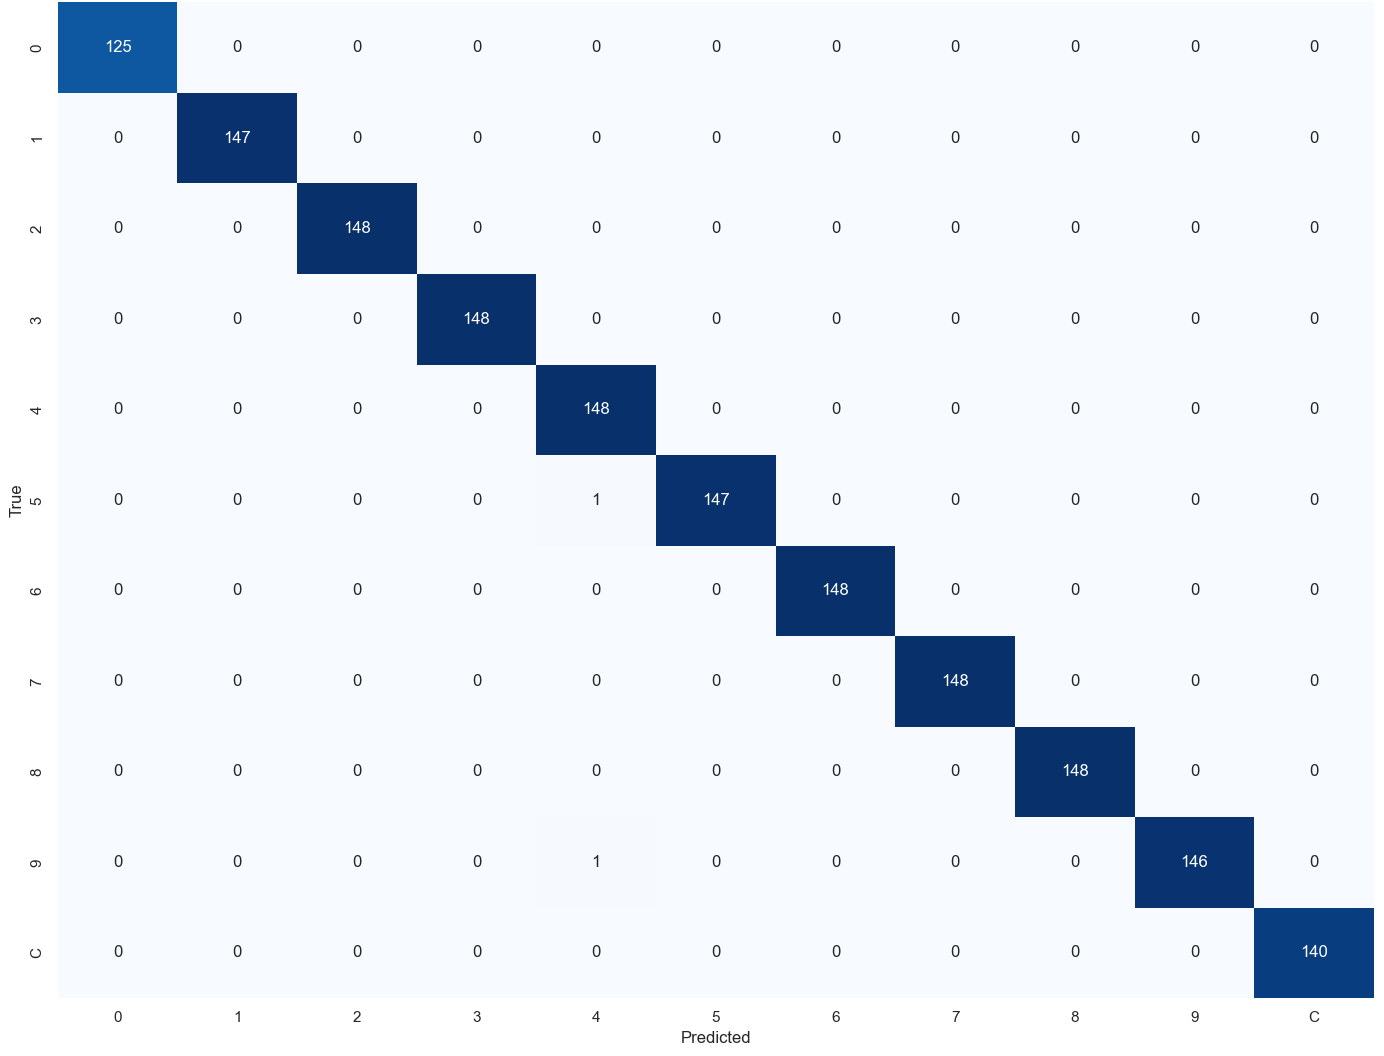
\includegraphics[width=\columnwidth]{image2.png}
  \caption{SVM (RBF) -- One Hand.}
  \label{fig:cm_one}
\end{figure}

\begin{figure}[H]
  \centering
  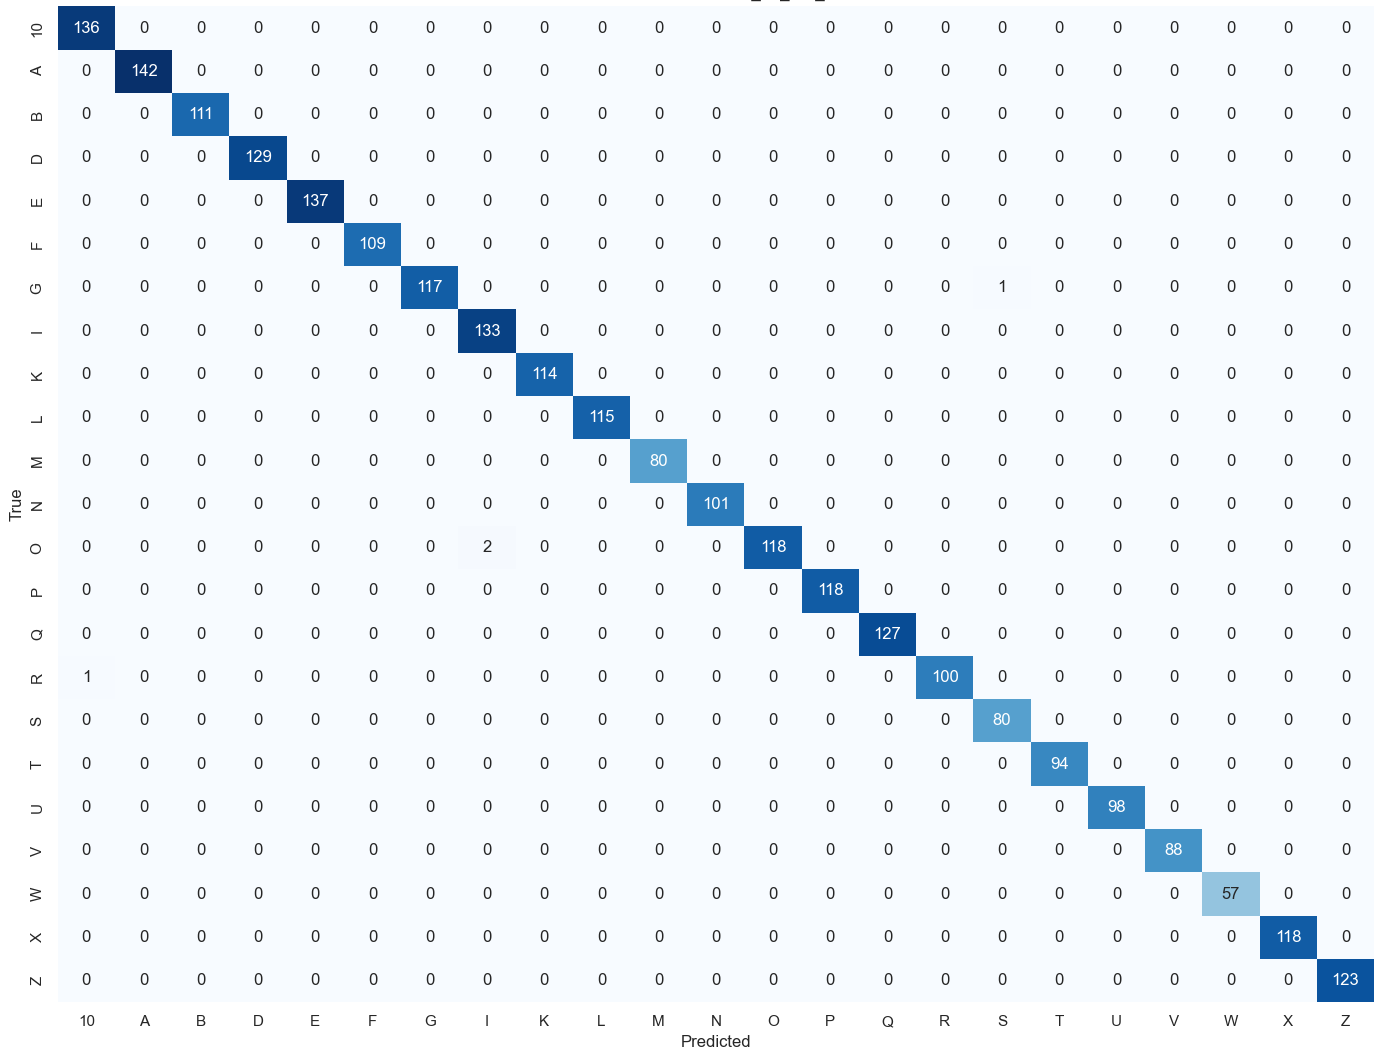
\includegraphics[width=\columnwidth]{image1.png}
  \caption{SVM (RBF) -- Two Hand.}
  \label{fig:cm_two}
\end{figure}

\end{document}
